\documentclass[11pt,table,compress]{beamer}
\usetheme{Warsaw}
\usecolortheme{dolphin}
\usepackage[utf8]{inputenc}
\usepackage[spanish]{babel}
\usepackage{amsmath}
\usepackage{amsfonts}
\usepackage{amssymb}
\usepackage{graphicx}
\usepackage{multirow}
\usepackage{physics}
%\usepackage[table]{xcolor}
\author{Cindy Castellón}
\title[Defensa final]{\textbf{Trabajo de investigación:} \\ \textit{Simulaciones de chubascos atmosféricos producidos por UHECR con diferentes composiciones}.} 
%\setbeamercovered{transparent} 
\setbeamertemplate{navigation symbols}{} 
%\logo{} 
\institute{Escuela de Física} 
%\date{} 
\subject{Investigación en Física} 

\begin{document}

\begin{frame}
\titlepage
\end{frame}

\begin{frame}
\tableofcontents
\end{frame}

\section{Marco Teórico}
	\subsection{Sustento histórico}
	\begin{frame}{Rayos cósmicos}
		\begin{columns}
			\begin{column}{0.35\textwidth}
				\begin{block}{ }
				Descubiertos por Victor Hess en 1912; son partículas cargadas originadas en ambientes extremos del universo que llegan a la 						Tierra con altas energías ($>10^9$ eV).
				\end{block}
			\end{column}
			\begin{column}{0.65\textwidth}
				\begin{figure}
				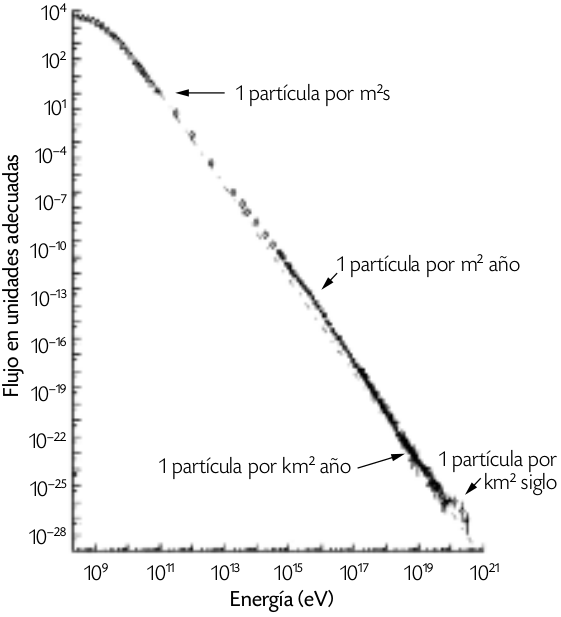
\includegraphics[width=0.9\textwidth, height=0.6\textheight]{Figuras/espectro_RC} 
				\caption{Intensidad del flujo de rayos cósmicos en función de su energía. Es representado por una ley de potencias $E^{-2.7}$ 						(, 1999).}
				\end{figure}				
			\end{column}			
		\end{columns}	
	\end{frame}
	
	\begin{frame}{Chubascos atmosféricos}
		\begin{figure}
		\centering
		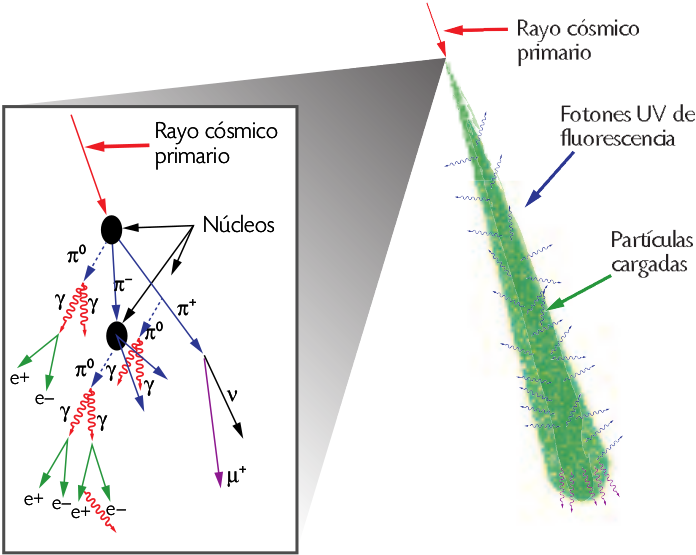
\includegraphics[width=0.7\textwidth]{Figuras/air_shower} 
		\caption{Esquema de la formación y desarrollo de un chubasco atmosférico. Se ilustra la componente hadrónica y la electromagnética. 				(ALguien, 1999)}
		\label{fig:airshower}
		\end{figure}	
	\end{frame}	
	
	\begin{frame}{Modelos de chubascos}
		\begin{block}{Sección eficaz}
		Probabilidad de que una partícula interactúe.
		\end{block}	
		\vspace{5 mm}
		\begin{block}{Multiplicidad}
		Número de mesones producidos en una interacción hadrónica.
		\end{block}	
		\vspace{5 mm}
		\begin{block}{Inelasticidad}
		Fracción de la energía que se invierte en producción de mesones.
		\end{block}			
	\end{frame}		
	
	
	\subsection{Estado del conocimiento}
	\begin{frame}{Estado del conocimiento}
	Preguntas abiertas en la física de rayos cósmicos: \vspace{4 mm}
		\begin{itemize}
		\item ¿Cómo alcanzan sus altas energías observadas? \vspace{3 mm}
		\item ¿Dónde se producen?\vspace{3 mm}
		\item A ultraaltas energías ¿qué especie de partículas son?
		\end{itemize}
	\end{frame}
	
	\begin{frame}
		\begin{figure}
		\centering
		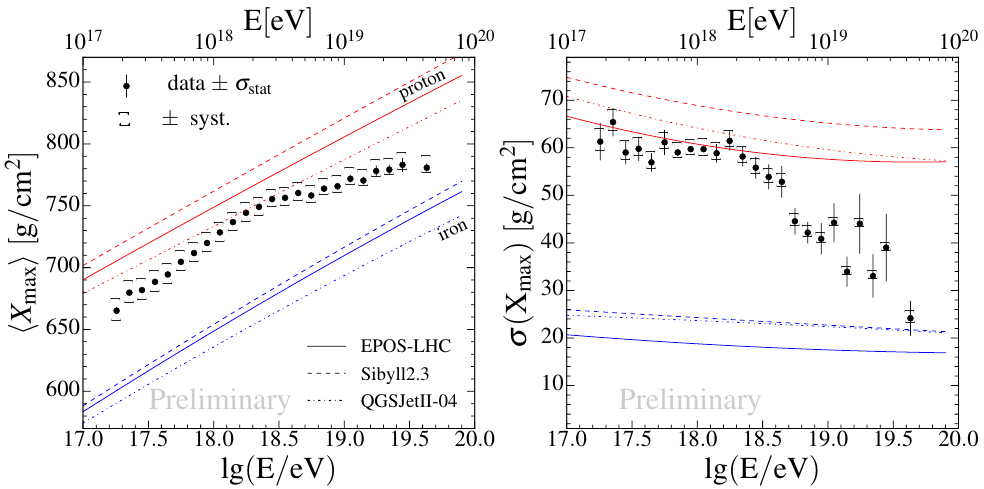
\includegraphics[width=\textwidth]{Figuras/Xmax_Bellido} 
		\caption{$X_{max}$ promedio (izquierda) y desviación estándar (derecha) de chubascos simulados con diferentes modelos hadrónicos (Bellido, 2017).}
		\end{figure}	
	\end{frame}

	\begin{frame}
		\begin{figure}
		\centering
		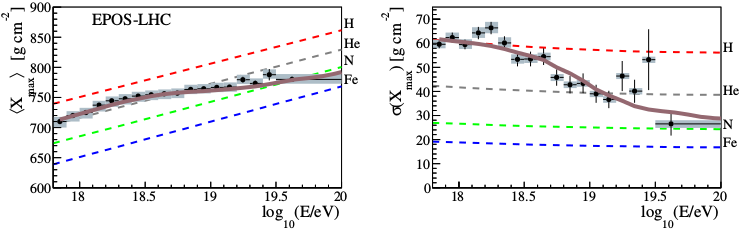
\includegraphics[width=\textwidth]{Figuras/Xmax_PAO} 
		\caption{$X_{max}$ promedio (izquierda) y desviación estándar (derecha) asumiendo una composición mixta (línea sólida), comparado con datos del Observatorio Pierre Auger (Sciutto, 2019).}
		\end{figure}	
	\end{frame}
	
	\begin{frame}
		\begin{figure}[]
		\centering
		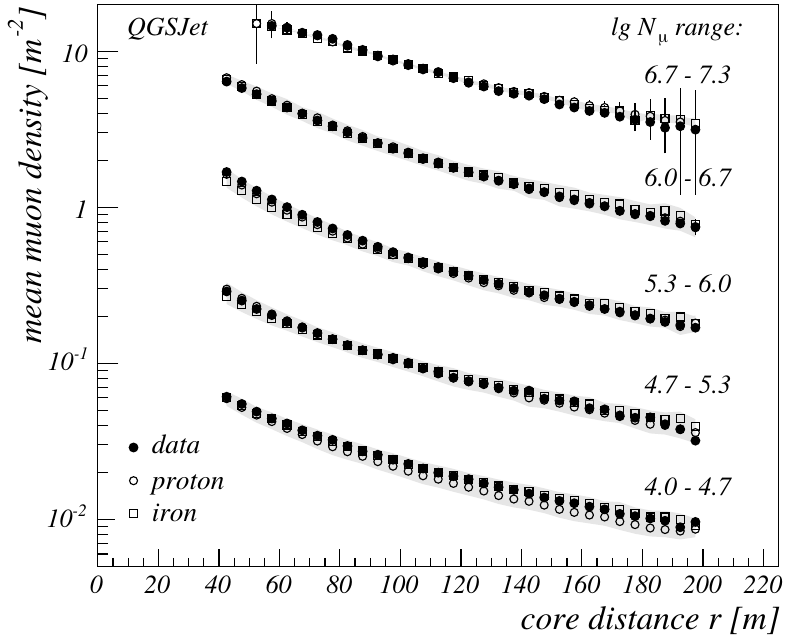
\includegraphics[width=0.6\textwidth]{Figuras/Apel2005} 
		\caption{Comparación de distribuciones laterales de muones resultado de simulaciones con el programa CORSIKA y medidas del observatorio KASCADE (Apel et al, 2005).}
		\label{fig:Apel}
		\end{figure}
	\end{frame}
	
\section{Objetivos}
\begin{frame}{Objetivos}
	\begin{enumerate}
		\item Verificar el efecto de una composición mixta de los UHECR en la profundidad del máximo $X_{\text{max}}$. \vspace{0.5cm}
		
		\item Analizar las distribuciones laterales y densidad de partículas (electrones y muones) a una distancia fija del eje en chubascos 				producidos por diferentes composiciones primarias. \vspace{0.5cm}
		
		\item Examinar las discrepancias entre las predicciones realizadas con los diferentes modelos hadrónicos de altas energías.
	\end{enumerate}	
\end{frame}

\section{Metodología}
\begin{frame}{Metodología}
Con el sistema AIRES se simularon chubascos producidos por rayos cósmicos de energías entre $10^{17}$ y $10^{20}$ eV, en la ubicación de Malargue en Mendoza, Argentina -donde se encuentra una de las estaciones del Observatorio Pierre Auger-. \\ \vspace{0.5 cm}

Se consideraron direcciones de incidencia con ángulo zenital entre 0$^{o}$ y 70$^{o}$ y ángulo azimutal distribuido isotrópicamente entre 0$^{o}$ y 360$^{o}$. \\ \vspace{0.5 cm}

Se utilizaron tres modelos de interacciones hadrónicas de altas energías; Sibyll 2.3c, EPOS-LHC y QGSJETII-04.
\end{frame}

\begin{frame}
	\begin{figure}
	\centering
	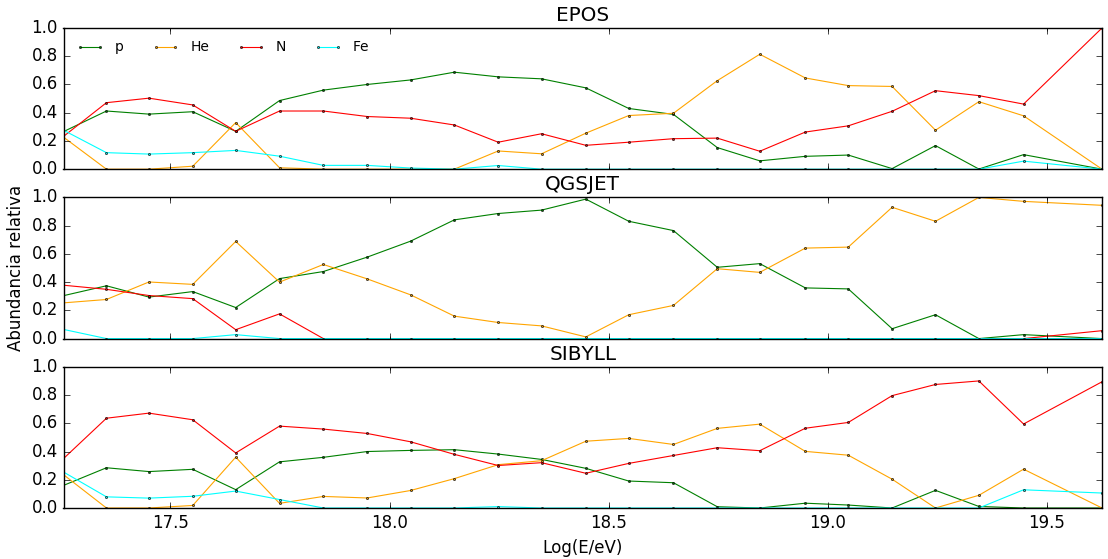
\includegraphics[width=\textwidth,height=0.7\textheight]{Figuras/composition} 
	\caption{Composición en función de la energía, resultado de ajustes con los datos de $X_{\text{max}}$ del Observatorio Pierre Auger 				realizados con tres modelos de interacciones hadrónicas de altas energías.}
	\label{fig:composition}
	\end{figure}	
\end{frame}

\begin{frame}
En síntesis, el sistema AIRES consiste de:\vspace{0.3 cm}
	\begin{itemize}
	\item Los programas de simulación principales (AiresEPLHC, AiresEP199, AiresQIIr03, AiresQIIr04, AiresS21, AiresS23, AiresS23c), cada uno 			conteniendo la interfaz para un paquete de interacciones hadrónicas. \vspace{0.3 cm}
	\item El programa resumen (AiresSry), diseñado para procesar parte de los datos generados por los programas de simulación. \vspace{0.3 cm}
	\item El programa de conversión de formato IDF (\textit{internal dump file}) a ADF (\textit{portable dump file}) (AiresIDF2ADF). \vspace{0.3 		cm}
	\item Una librería de auxiliares para procesar los archivos de salida de los programas de simulación (libAires.a). \vspace{0.3 cm}
	\item El \textit{AIRES runner system}, para facilitar el trabajo con AIRES en ambientes UNIX. \vspace{0.3 cm}
	\end{itemize}
\end{frame}

\section{Resultados}
\begin{frame}{Resultados}
Se muestran y discuten resultados de: \vspace{5 mm}
	\begin{itemize}
	\item Profundidad del máximo $X_{max}$. Composición ligera, pesada y mixta. \vspace{3 mm}
	\item Distribuciones laterales de electrones y muones. Composición ligera y pesada.\vspace{3 mm}
	\item Densidad de electrones y muones a 1000 m. Composición ligera y pesada.
	\end{itemize}
 \end{frame}

	\subsection[$X_{max}$]{Profundidad del máximo}
	\begin{frame}{$X_{max}$}
		\begin{figure}
		\centering
		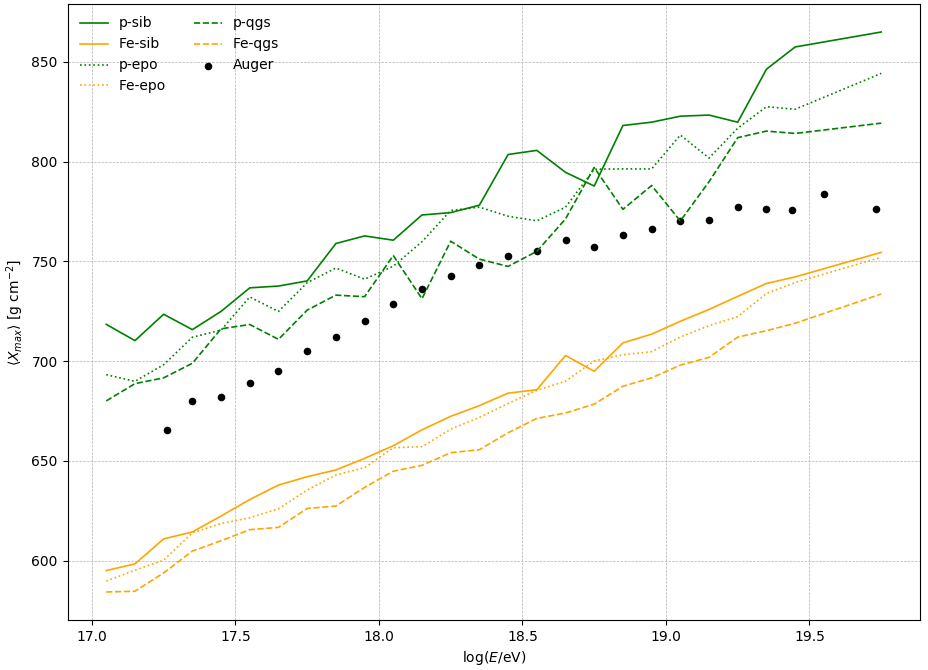
\includegraphics[width=0.8\textwidth]{Figuras/Xmax_pFe} 
		\caption{$X_{max}$ promedio de chubascos de composición ligera y pesada, simulados con diferentes modelos hadrónicos.}
		\end{figure}
	\end{frame}
	
	\begin{frame}
	Ajuste lineal:
		\begin{align*}
		\langle X_{max} \rangle = \Lambda \log(E) + b
		\end{align*}
	\begin{table}[] 
	\centering
	\caption{Parámetros del ajuste lineal a los datos de $X_{\text{max}}$ de diferentes modelos y composiciones.}
		\begin{tabular}{c|c|cc}
		\hline
		Modelo                       &  Prim  	& $\Lambda$ 	& $b$      \\ \hline
		\multirow{2}{*}{Sibyll 2.3c} & 	p  		& 58.133    	& -284.299 \\  
		                             & 	Fe 		& 60.589    	& -435.177 \\ \hline
		\multirow{2}{*}{EPOS-LHC}    & 	p  		& 56.129    	& -262.527 \\  
		                             & 	Fe 		& 60.731    	& -443.335 \\ \hline
		\multirow{2}{*}{QGSJETII-04} & 	p  		& 52.319    	& -206.041 \\ 
		                             & 	Fe 		& 56.287    	& -374.749 \\ \hline
		\end{tabular}
	\label{linear_params}
	\end{table}
	\end{frame}
	
	\begin{frame}
		\begin{figure}[] 
			\centering
			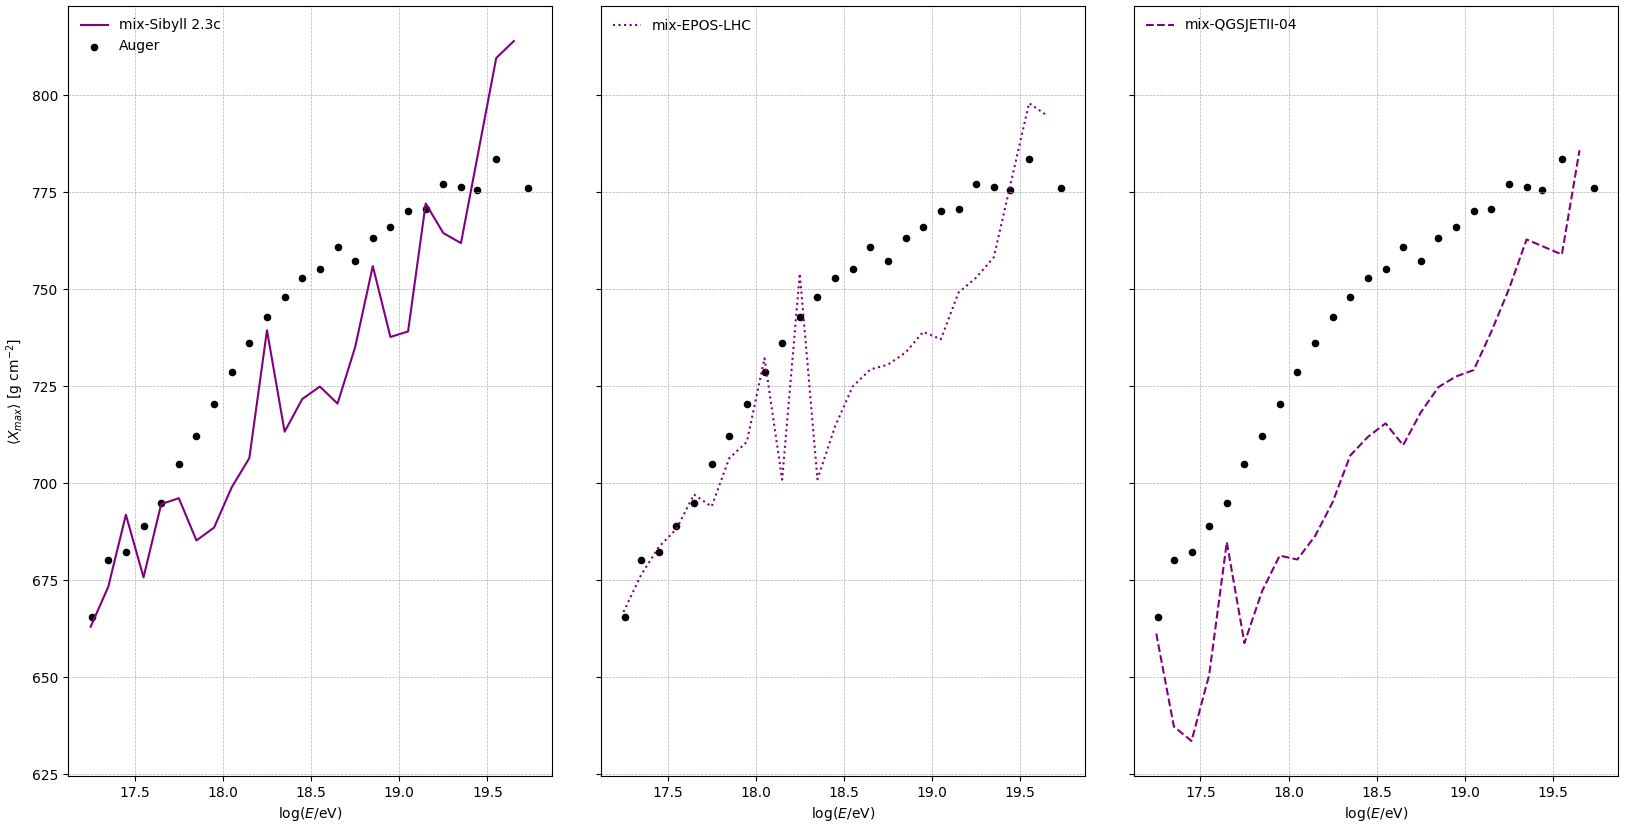
\includegraphics[width=\textwidth, height=0.7\textheight]{Figuras/Xmax_mix}
			\caption{Resultados de la profundidad del máximo en chubascos con composición primaria mixta, comparándolos con datos experimentales del Observatorio Pierre Auger.}
			\label{fig:xmax_mix}
		\end{figure}
	\end{frame}			
	
	\subsection[Distribuciones]{Distribuciones laterales}
	\begin{frame}{Distribuciones laterales}
	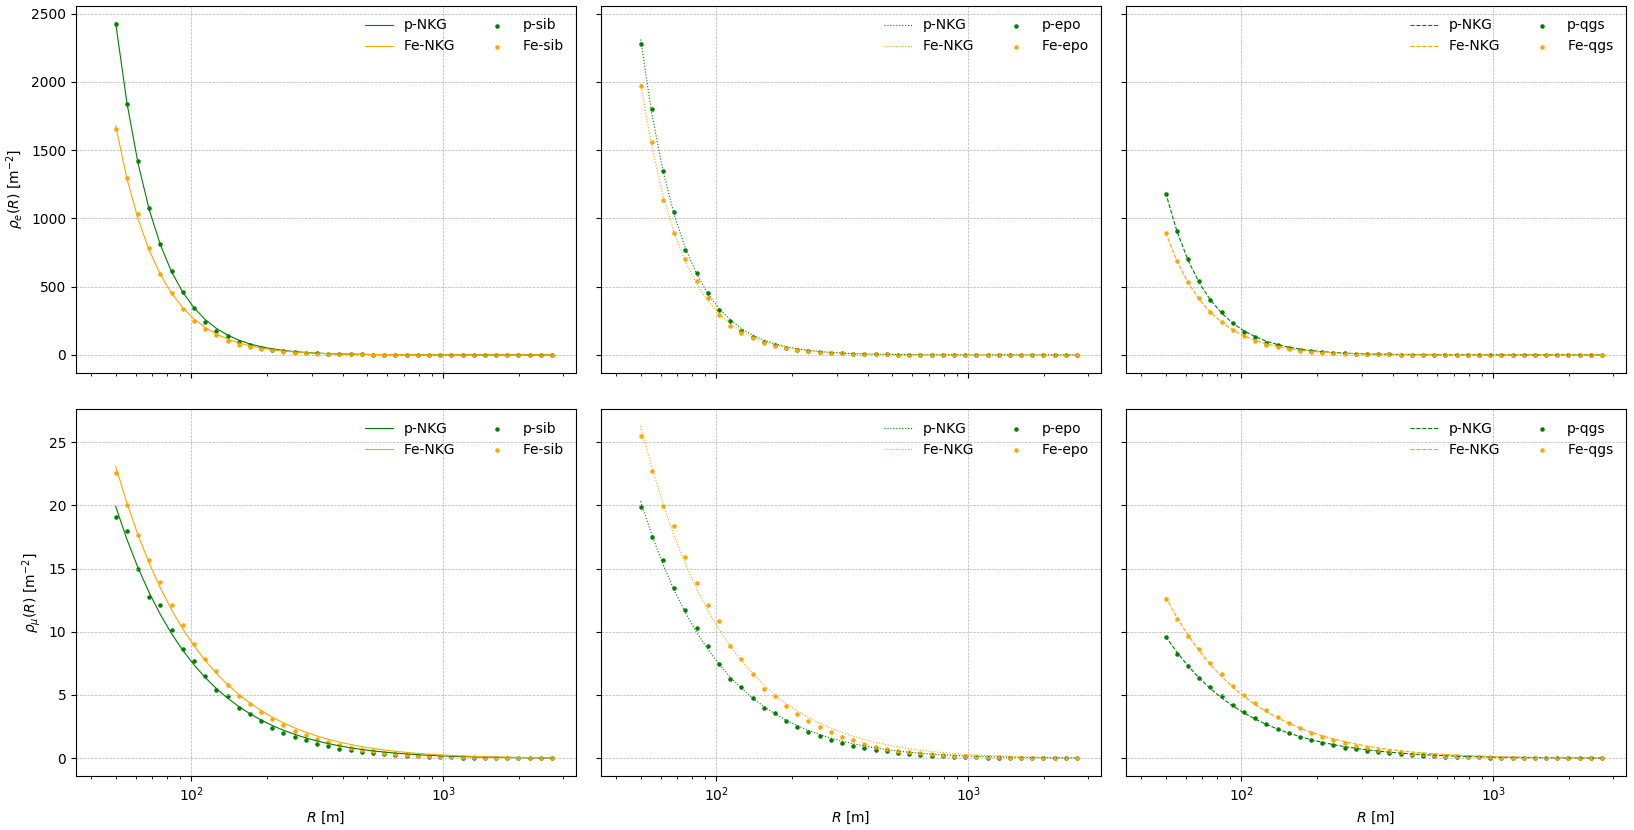
\includegraphics[height=0.8\textheight, width=\textwidth]{Figuras/distlat_pFe}
	\end{frame}
	
	\begin{frame}
	Los resultados se ajustaron a una función NKG modificada de la forma:
		\begin{align*}
		\rho(r) = c \qty(\frac{r}{r_{opt}})^{-\beta}\qty(1-\frac{r}{r_{opt}})^{-\beta}.
		\end{align*}
		\begin{columns}
			\begin{column}{0.5\textwidth}
				\begin{table}
				\caption{Parámetros para distribución de electrones}
				\begin{tabular}{c|c|cc}
				\hline
						                     &  & c     & $\beta$ \\ \hline
				\multirow{2}{*}{Sib} & p        & 1.313 & 2.553   \\  
				                             & Fe       & 1.339 & 2.421   \\ \hline
				\multirow{2}{*}{EPO}    & p        & 1.437 & 2.505   \\  
				                             & Fe       & 1.390 & 2.465   \\ \hline
				\multirow{2}{*}{QGS} & p        & 0.757 & 2.497   \\ 
				                             & Fe       & 0.691 & 2.432   \\ \hline
				\end{tabular}
				\end{table}
			\end{column}
			\begin{column}{0.5\textwidth}
				\begin{table}
				\caption{Parámetros para distribución de muones}
				\begin{tabular}{c|c|cc}
				\hline
				                     		 &  & c     & $\beta$ \\ \hline
				\multirow{2}{*}{Sib} & p        & 0.436 & 1.297   \\ 
				                             & Fe       & 0.586 & 1.247   \\ \hline
				\multirow{2}{*}{EPO}    & p        & 0.425 & 1.313   \\  
				                             & Fe       & 0.684 & 1.238   \\ \hline
				\multirow{2}{*}{QGS} & p        & 0.212 & 1.295   \\  
				                             & Fe       & 0.318 & 1.253   \\ \hline
				\end{tabular}
				\end{table}
			\end{column}
		\end{columns}
	\end{frame}	
	
	\begin{frame}
		\begin{figure}[] 
		\centering
		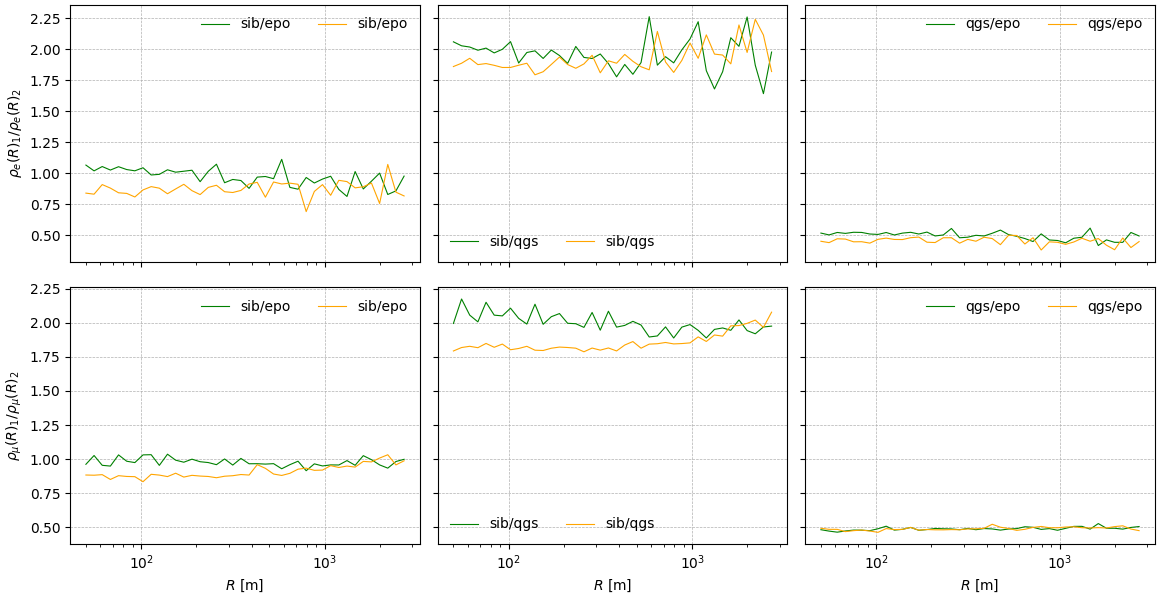
\includegraphics[width=\textwidth]{Figuras/distlat_models}
		\caption{Razones entre densidades de partículas de pares de modelos de interacción hadrónica.}
		\label{fig:distlat_modelos}
		\end{figure}
	\end{frame}
	
	\begin{frame}
	Se graficaron las distribuciones laterales para tres subintervalos de energía designados como $bin02$, $bin13$ y $bin24$, con energías
\begin{align*}
10^{17.1} \leq & E_{bin03} < 10^{17.2} \text{ eV}, \\
10^{18.2} \leq & E_{bin14} < 10^{18.3} \text{ eV}, \text{ y}\\
10^{19.7} \leq & E_{bin23} < 10^{19.8} \text{ eV}.
\end{align*}
	\end{frame}
	
	\begin{frame}
		\begin{figure}[h] 
		\centering
		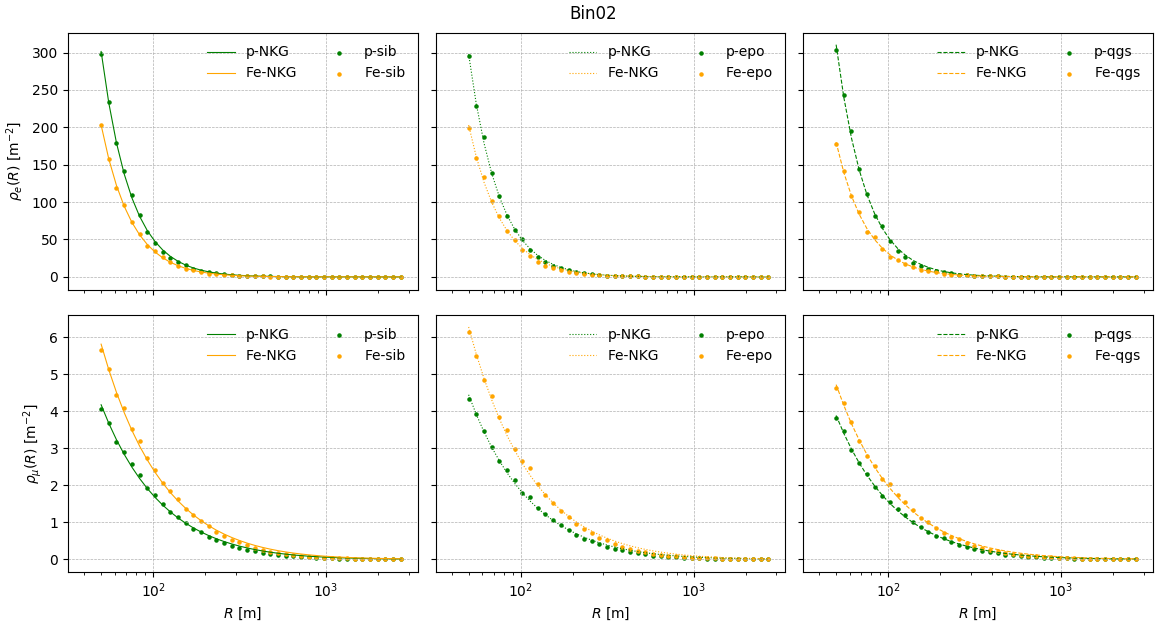
\includegraphics[height=0.7\textheight, width=\textwidth]{Figuras/distlat_bin02}
		\caption{Distribuciones laterales de electrones y muones resultado de chubascos de energía promedio $E=10^{17.15}$ eV.}
		\label{fig:distlat_bin02}
		\end{figure}
	\end{frame}
	
	\begin{frame}
		\begin{figure}[] 
		\centering
		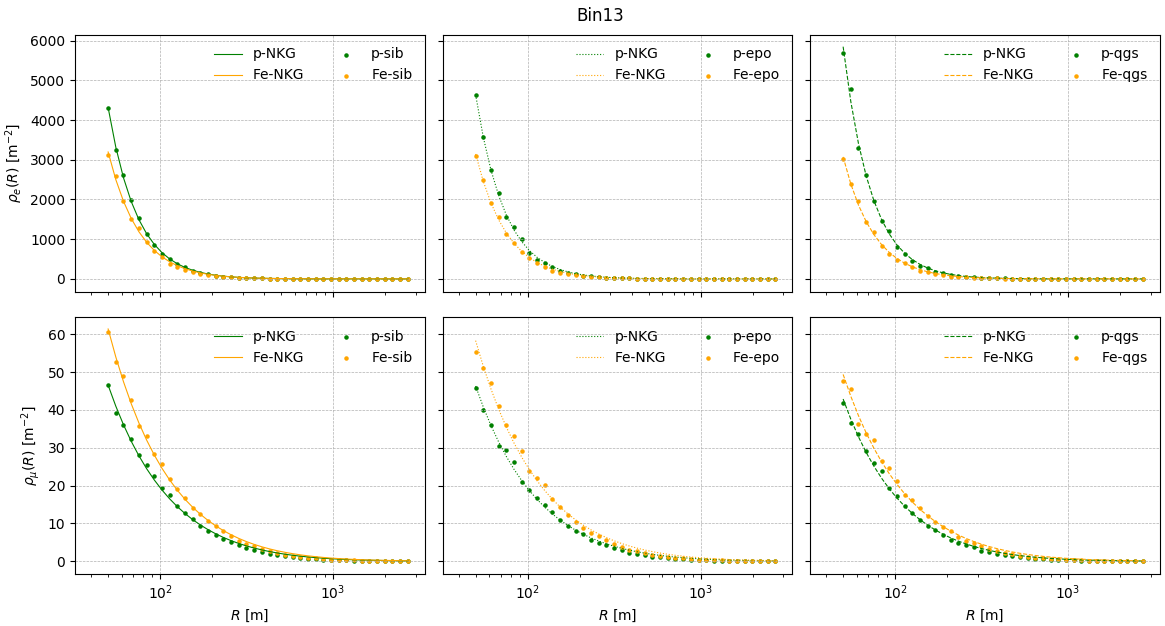
\includegraphics[height=0.7\textheight, width=\textwidth]{Figuras/distlat_bin13}
		\caption{Distribuciones laterales de electrones y muones resultado de chubascos de energía promedio $E=10^{18.25}$ eV.}
		\label{fig:distlat_bin13}
		\end{figure}
	\end{frame}		
		
	\begin{frame}	
		\begin{figure}[] 
		\centering
		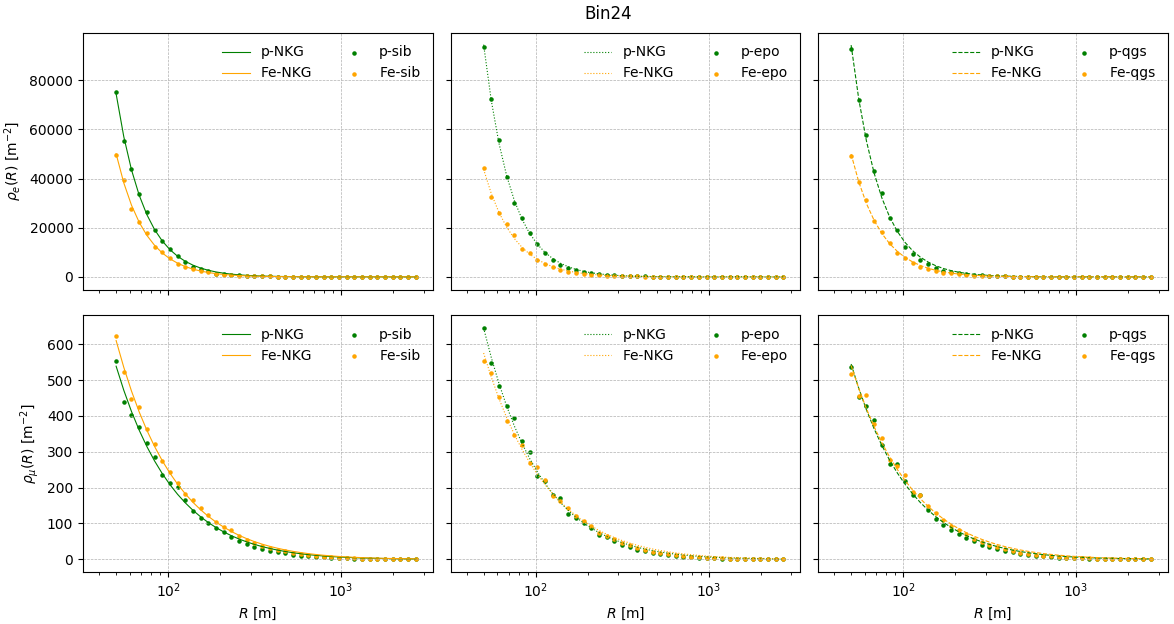
\includegraphics[height=0.7\textheight, width=\textwidth]{Figuras/distlat_bin24}
		\caption{Distribuciones laterales de electrones y muones resultado de chubascos de energía promedio $E=10^{19.75}$ eV.}
		\label{fig:distlat_bin24}
		\end{figure}
	\end{frame}
	
	\begin{frame}
	\begin{footnotesize}
	
		\begin{table}[] 
		\centering
		\caption{Parámetros del ajuste de la distribución de electrones y muones.}	
		\begin{tabular}{cc|cc|cc|cc}
		\hline
		\multicolumn{2}{c|}{Subintervalo}                          & \multicolumn{2}{c|}{$bin02$} & \multicolumn{2}{c|}{$bin13$} & \multicolumn{2}{c}{$bin24$} \\ \hline
		\multicolumn{1}{c|}{Modelo}                       & Prim. & $c$          & $\beta$       & $c$          & $\beta$       & $c$          & $\beta$       \\ \hline
		\multicolumn{1}{c|}{\multirow{2}{*}{Sibyll 2.3c}} & p     & 0.242        & 2.419         & 3.154        & 2.450         & 48.247       & 2.491         \\
		\multicolumn{1}{c|}{}                             & Fe    & 0.193        & 2.362         & 3.811        & 2.284         & 30.944       & 2.507         \\ \hline
		\multicolumn{1}{c|}{\multirow{2}{*}{EPOS-LHC}}    & p     & 0.282        & 2.362         & 3.433        & 2.446         & 48.576       & 2.570         \\
		\multicolumn{1}{c|}{}                             & Fe    & 0.319        & 2.191         & 3.423        & 2.315         & 38.819       & 2.385         \\ \hline
		\multicolumn{1}{c|}{\multirow{2}{*}{QGSJETII-04}} & p     & 0.270        & 2.392         & 3.577        & 2.511         & 61.917       & 2.487         \\
		\multicolumn{1}{c|}{}                             & Fe    & 0.171        & 2.361         & 3.140        & 2.336         & 42.061       & 2.402         \\ \hline
		
		
		\end{tabular}
		\label{edistlat_binparams}
		\end{table}	
		\begin{table}[] 
			\centering
			\begin{tabular}{cc|cc|cc|cc}
			\hline
			\multicolumn{2}{c|}{Subintervalo}                          & \multicolumn{2}{c|}{$bin02$} & \multicolumn{2}{c|}{$bin13$} & \multicolumn{2}{c}{$bin24$} \\ \hline
			\multicolumn{1}{c|}{Modelo}                       & Prim. & $c$          & $\beta$       & $c$          & $\beta$       & $c$          & $\beta$       \\ \hline
			\multicolumn{1}{c|}{\multirow{2}{*}{Sibyll 2.3c}} & p     & 0.124        & 1.193         & 1.431        & 1.182         & 13.841       & 1.243         \\
			\multicolumn{1}{c|}{}                             & Fe    & 0.179        & 1.181         & 1.811        & 1.196         & 16.816       & 1.219         \\ \hline
			\multicolumn{1}{c|}{\multirow{2}{*}{EPOS-LHC}}    & p     & 0.135        & 1.185         & 1.397        & 1.188         & 15.138       & 1.273         \\
			\multicolumn{1}{c|}{}                             & Fe    & 0.205        & 1.161         & 1.968        & 1.150         & 18.815       & 1.161         \\ \hline
			\multicolumn{1}{c|}{\multirow{2}{*}{QGSJETII-04}} & p     & 0.101        & 1.238         & 1.135        & 1.233         & 13.823       & 1.247         \\
			\multicolumn{1}{c|}{}                             & Fe    & 0.147        & 1.178         & 1.622        & 1.159         & 17.012       & 1.174         \\ \hline
			\end{tabular}
			\label{mudistlat_binparams}
		\end{table}
 		\end{footnotesize}

	\end{frame}
			
	\subsection[Densidad a $r_{opt}$]{Densidad de partículas a $r_{opt}$}
	\begin{frame}{Densidad de partículas a $r_{opt}$}
		\begin{figure}[h] 
		\centering
		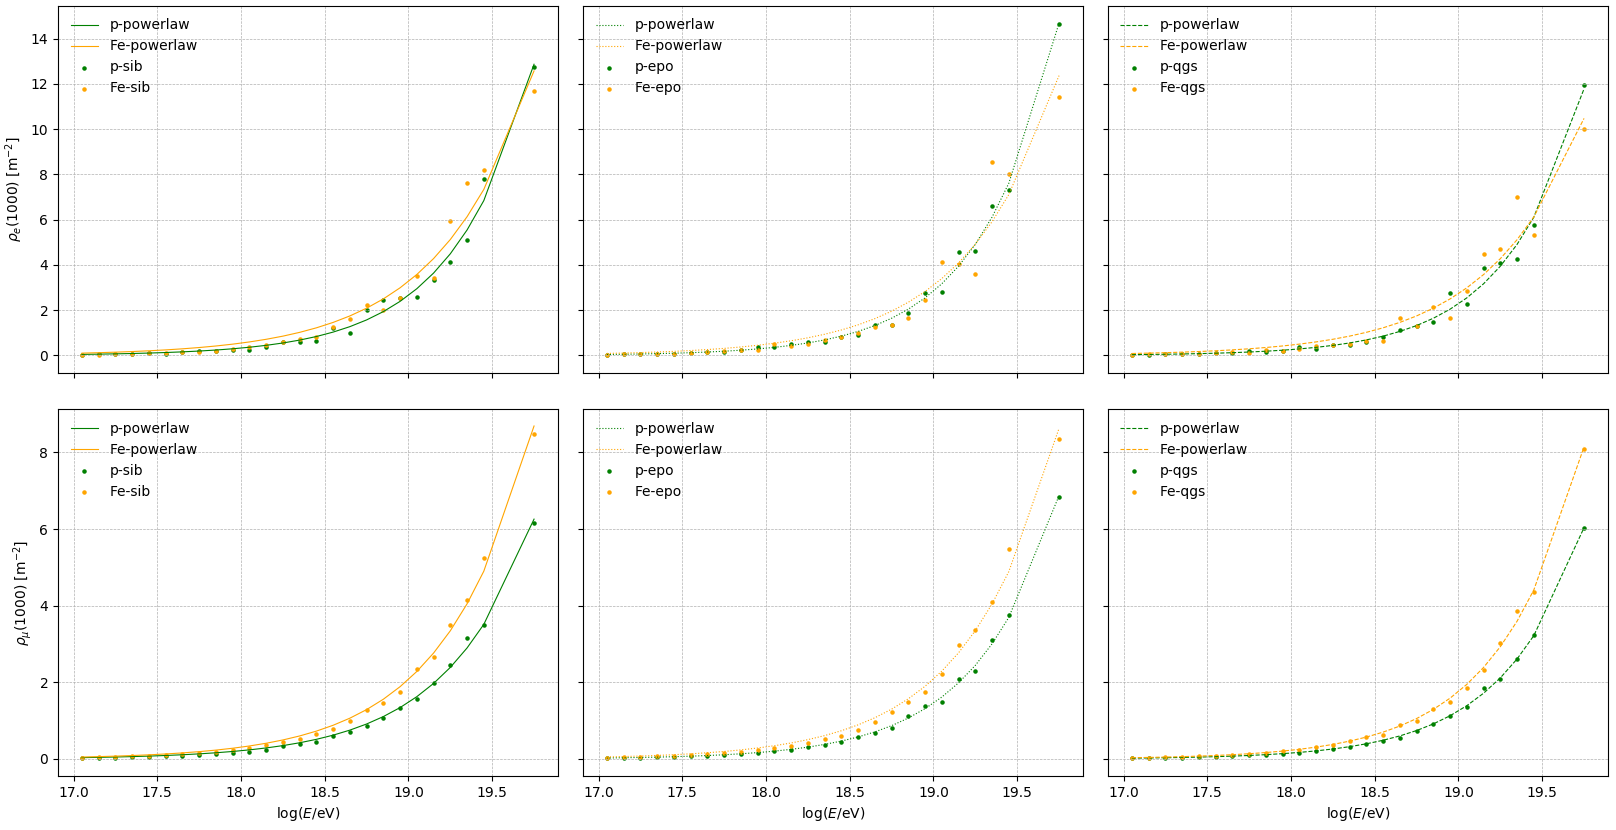
\includegraphics[height=0.7\textheight, width=\textwidth]{Figuras/density_pFe}
		\caption{Densidad de partículas (electrones y muones) a una distancia $R=r_{opt}$ en función de la energía inicial}
		\label{fig:density}
		\end{figure}
	\end{frame}
	
	\begin{frame}
	Ajuste a una ley de potencias:
	\begin{align*} \label{powerlaw}
	\rho_{r_{opt}}(E) = a \qty(\frac{E}{10^{18}})^b.
	\end{align*}
		\begin{columns}
			\begin{column}{0.5\textwidth}
				\begin{table}[] 
				\centering
				\caption{Parámetros del ajuste de la densidad de electrones.}
				\begin{tabular}{c|c|cc}
				                     &  & $a$ & $b$   \\ \hline
				\multirow{2}{*}{Sib} & p     & 0.323     & 0.915 \\
				                             & Fe    & 0.542     & 0.780 \\ \hline
				\multirow{2}{*}{EPO}    & p     & 0.317     & 0.952 \\
				                             & Fe    & 0.489     & 0.802 \\ \hline
				\multirow{2}{*}{QGS} & p     & 0.255     & 0.952 \\
				                             & Fe    & 0.454     & 0.779 \\ \hline
				\end{tabular}
				\label{edensity_params}
				\end{table}
			\end{column}
			\begin{column}{0.5\textwidth}
				\begin{table}[] 
				\centering
				\caption{Parámetros del ajuste de la densidad de muones.}
				\begin{tabular}{c|c|cc}
				                   &  & $a$ 		 & $b$   \\ \hline
				\multirow{2}{*}{Sib} & p     & 0.215     & 0.836 \\
				                             & Fe    & 0.308     & 0.829 \\ \hline
				\multirow{2}{*}{EPO}    & p     & 0.184     & 0.898 \\
				                             & Fe    & 0.314     & 0.822 \\ \hline
				\multirow{2}{*}{QGS} & p     & 0.154     & 0.911 \\
				                             & Fe    & 0.227     & 0.888 \\ \hline
				\end{tabular}
				\label{mudensity_params}
				\end{table}
			\end{column}
		\end{columns}
	\end{frame}

\section{Conclusiones}
\begin{frame}{Conclusiones}
	\begin{itemize}
	\item La hipótesis de la composición mixta es apoyada por los resultados de $X_{\text{max}}$. \vspace{3 mm}
	\item El modelo EPOS-LHC el que más acertadamente reproduce los datos observacionales de $X_{max}$. el modelo QGSJETII-04 el que predice menores profundidades.
	\end{itemize}
\end{frame}

\begin{frame}
	\begin{itemize}
	\item En el caso de las distribuciones laterales en todo el intervalo de energías, los tres modelos producen formas similares. QGSJETII-04 muestra menor densidad de partículas.\vspace{3 mm}
	\item Se observa que al aumentar la energía la forma de las distribuciones se mantiene similar, aumentando en general el número de partículas. \vspace{3 mm}
	\item El efecto de la composición primaria es contrario para electrones y muones. A altas energías primarias las distribuciones de distintas composiciones casi se sobrelapan.
	\end{itemize}
\end{frame}

\begin{frame}
	\begin{itemize}
	\item Las densidades de partículas a la distancia óptima del PAO en función de la energía inicial no muestran una clara dependencia del modelo de interacciones hadrónicas.\vspace{3 mm}
	
	\item La densidad de electrones no presenta dependencia tampoco de la composición primaria, mientras que la densidad de muones aumenta sus diferencias entre composiciones al aumentar la energía.
	\end{itemize}
\end{frame}

\end{document}
